% ============================================================
% Corrigé du TD : Séries de Fourier
% Pôle Formation UIMM - CVDL - BTS Industriel - S. JAUBERT
% Compiler d abord le cours et le TD (fichiers .aux), puis ce corrigé (deux passes).
% ============================================================
\documentclass[a4paper,11pt]{article}
\usepackage[utf8]{inputenc}
\usepackage[T1]{fontenc}
% babel-french absent sur certains postes : chargement conditionnel
\IfFileExists{french.ldf}{\usepackage[french]{babel}}{}
\usepackage{helvet}
\usepackage{courier}
\renewcommand{\familydefault}{\sfdefault}
\usepackage[top=3cm, bottom=2.5cm, left=2cm, right=2cm, headheight=2cm]{geometry}
\usepackage{amsmath,amssymb,amsfonts}
\usepackage{graphicx}
\usepackage[dvipsnames,table]{xcolor}
\usepackage{tikz}
\usepackage{pgfplots}
\pgfplotsset{compat=1.18}
\usepackage[most]{tcolorbox}
\usepackage{fancyhdr}
\usepackage{enumitem}
\usepackage{array,needspace}
\usepackage{titlesec}
\usepackage{xr-hyper}
\usepackage{hyperref}
\externaldocument[C-]{MOD13_Series_Fourier_Cours_v1_0}
\externaldocument[T-]{MOD13_Series_Fourier_TD_v1_0}

\definecolor{uimmblue}{HTML}{005C85}
\definecolor{uimmred}{HTML}{D31326}
\definecolor{uimmlightblue}{HTML}{E8F1F8}
\definecolor{uimmgray}{HTML}{333333}
\definecolor{uimmlightgray}{HTML}{F5F5F5}
\hypersetup{colorlinks=true, linkcolor=uimmblue, urlcolor=uimmblue}

\titleformat{\section}{\Large\bfseries\color{uimmblue}}{}{0pt}{}[\vspace{2pt}{\color{uimmblue}\titlerule[1.2pt]}]
\setlist[enumerate,1]{label={\color{uimmblue}\textbf{\arabic*.}}}
\setlist[enumerate,2]{label=\alph*)}
\setlist[itemize,1]{label={\color{uimmblue}\textbullet}}

\newtcolorbox{correction}[1][]{%
  colback=green!5, colframe=green!50!black,
  fonttitle=\bfseries\color{white}, title={\textsf{Correction}~#1},
  coltitle=white, boxrule=1pt, arc=3pt,
  left=8pt, right=8pt, top=6pt, bottom=6pt, before skip=8pt, after skip=8pt, breakable}
\newtcolorbox{piege}{%
  colback=uimmred!5, colframe=uimmred!80!black, boxrule=1pt, arc=3pt,
  left=8pt, right=8pt, top=5pt, bottom=5pt, before skip=6pt, after skip=6pt}

\newcommand{\M}[1]{\begin{pmatrix}#1\end{pmatrix}}
% Référence vers le cours : §section, page
\newcommand{\cours}[1]{§\ref{C-#1} p.~\pageref{C-#1}}
% Ligne de références en tête de chaque correction
\newcommand{\source}[2]{{\footnotesize\color{uimmgray}\textbf{Réf.} \enspace Énoncé : TD MOD13 p.~\pageref{T-#1} \enspace$\bullet$\enspace Cours MOD13 : #2}\par\smallskip}
\newcommand{\annexe}[1]{annexe p.~\pageref{C-#1}}
\newcommand{\q}[1]{\textbf{\color{uimmblue}#1}\ }

\pagestyle{fancy}
\fancyhf{}
\renewcommand{\headrulewidth}{0pt}
\fancyhead[L]{\raisebox{-0.5\height}{
\includegraphics[height=1.5cm]{logo_uimm_placeholder.jpg}}}
\fancyhead[C]{\begin{minipage}{8cm}\centering
  {\small\color{uimmblue}\textbf{Pôle Formation UIMM - CVDL}}\\
  {\footnotesize\color{uimmgray} BTS Industriel -- Mathématiques}\end{minipage}}
\fancyhead[R]{{\small\color{uimmblue}\textbf{MOD13 -- Corrigé TD}}}
\fancyfoot[C]{{\color{uimmblue}\rule{\textwidth}{1pt}}\\[2pt]
  {\footnotesize\color{uimmgray} Pôle Formation UIMM -- Centre-Val de Loire \hfill S. JAUBERT \hfill \thepage}}

\begin{document}

\begin{tcolorbox}[colback=uimmblue, colframe=uimmblue, sharp corners, boxrule=0pt,
  left=14pt, right=14pt, top=10pt, bottom=10pt]
{\color{white}\LARGE\bfseries Corrigé -- Travaux Dirigés MOD13}\\[4pt]
{\color{white}\large Séries de Fourier}
\end{tcolorbox}

\begin{tcolorbox}[colback=uimmlightgray, colframe=uimmgray, boxrule=0.8pt, arc=3pt]
\small\textbf{Mode d'emploi.} Chaque correction indique la page de l'énoncé dans le TD et le paragraphe du cours à relire (numéro de paragraphe et page du support de cours MOD13). Les encadrés rouges signalent les erreurs les plus fréquentes.
\end{tcolorbox}

% ============================================================
\needspace{8cm}
\section{Séries numériques}

\begin{correction}[-- Exercice 1 : séries géométriques]
\source{exo:1}{\cours{th:geometrique}}
\q{(a)} $q = \frac13$, $|q|<1$ : converge, somme $\dfrac{1}{1-\frac13} = \dfrac32$.
\q{(b)} $q = 1{,}02\geq 1$ : diverge.
\q{(c)} $q = -0{,}5$, $|q|<1$ : converge, somme $\dfrac{1}{1+0{,}5} = \dfrac23$.\\
\q{(d)} Premier terme $5$, $q = 0{,}6$ : converge, somme $\dfrac{5}{1-0{,}6} = 12{,}5$.
\q{(e)} La somme commence à $n = 1$ : premier terme $0{,}1$, $q = 0{,}1$ : converge, somme $\dfrac{0{,}1}{1-0{,}1} = \dfrac19$.
\begin{piege}
\textbf{Erreur fréquente :} appliquer $\frac{1}{1-q}$ quand la somme ne commence pas à $n = 0$. La formule sûre est « premier terme divisé par $1-q$ ».
\end{piege}
\end{correction}

\begin{correction}[-- Exercice 2 : vibration amortie du bâti d'une presse]
\source{exo:2}{\cours{th:geometrique} et \cours{ex:graisse}}
\q{a)} $D = \displaystyle\sum_{k=0}^{+\infty}4A_k = \sum_{k=0}^{+\infty}8\times 0{,}75^{k}$ : série géométrique de raison $0{,}75$, $|0{,}75|<1$, donc convergente.
\[
D = \frac{8}{1-0{,}75} = 32 \text{ mm.}
\]
Bien qu'il oscille indéfiniment en théorie, un point du bâti ne parcourt au total que $32$\,mm.

\q{b)} $2\times 0{,}75^{k} < 0{,}01 \iff 0{,}75^{k} < 0{,}005 \iff k > \dfrac{\ln 0{,}005}{\ln 0{,}75}\approx 18{,}4$ (on divise par $\ln 0{,}75 < 0$, ce qui change le sens). L'amplitude passe sous $0{,}01$\,mm à partir de $k = 19$, c'est-à-dire au $20$\textsuperscript{e} cycle.
\end{correction}

\begin{correction}[-- Exercice 3 : séries de Riemann et amplitudes d'harmoniques]
\source{exo:3}{\cours{subsec:riemann}}
\q{a)} $\sum\frac1{n^{1{,}5}}$ : $\alpha = 1{,}5 > 1$, converge. \quad $\sum\frac1{n^{0{,}8}}$ : diverge. \quad $\frac1{n\sqrt n} = \frac1{n^{1{,}5}}$ : converge. \quad $\sum\frac3{n^2} = 3\sum\frac1{n^2}$ : converge. \quad $\sum\frac1n$ : diverge ($\alpha = 1$).

\q{b)} $S_{10}\approx 1{,}5498$ ; $S_{100}\approx 1{,}6350$ ; $S_{1000}\approx 1{,}6439$ ; $\frac{\pi^2}{6}\approx 1{,}6449$. La convergence est lente : l'écart est d'environ $\frac1N$.

\q{c)} Créneau : la somme des amplitudes est infinie (termes en $\frac1n$, même en ne gardant que les $n$ impairs), mais la somme des carrés, en $\frac1{n^2}$, est finie. Triangle : les deux sommes sont finies (termes en $\frac1{n^2}$ et $\frac1{n^4}$). La puissance d'un signal, liée aux carrés des amplitudes (Parseval), est donc toujours finie.
\end{correction}

% ============================================================
\needspace{8cm}
\section{Signaux périodiques}

\begin{correction}[-- Exercice 4 : lire un signal]
\source{exo:4}{\cours{subsec:parite} et \cours{meth:expression}}
\begin{center}
\renewcommand{\arraystretch}{1.4}
\begin{tabular}{|c|c|c|p{2.4cm}|c|p{4.8cm}|}
\hline
\rowcolor{uimmlightblue}
Signal & Période & Fréquence & Parité & Moyenne & Expression \\
\hline
(A) & $20$\,ms & $50$\,Hz & ni paire ni impaire & $5$\,V & $10$ sur $]0\,;\,10[$, $0$ sur $]10\,;\,20[$ ($t$ en ms) \\
\hline
(B) & $0{,}5$\,s & $2$\,Hz & paire & $2$\,mm & $c(t) = 4 - 16t$ sur $[0\,;\,0{,}25]$ \\
\hline
(C) & $2$\,ms & $500$\,Hz & impaire & $0$\,A & $i(t) = 2t$ sur $]-1\,;\,1[$ ($t$ en ms) \\
\hline
\end{tabular}
\end{center}
Pour (B), la droite passe par $(0\,;\,4)$ et $(0{,}25\,;\,0)$ : $m = \frac{0-4}{0{,}25} = -16$. Pour (C), elle passe par $(-1\,;\,-2)$ et $(1\,;\,2)$ : $m = 2$, $p = 0$.
\end{correction}

\begin{correction}[-- Exercice 5 : courant redressé simple alternance]
\source{exo:5}{\cours{meth:representer} et \cours{subsec:coefficients}}
\q{a)} $\omega = \dfrac{2\pi}{0{,}02} = 100\pi\approx 314$\,rad/s.
\begin{center}
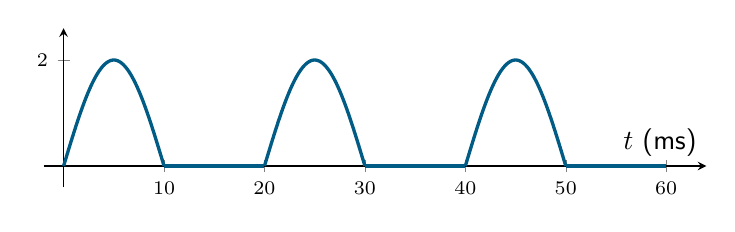
\begin{tikzpicture}
\begin{axis}[width=10cm, height=3.6cm, axis lines=middle, xlabel={$t$ (ms)}, xmin=-2, xmax=64, ymin=-0.4, ymax=2.6,
  xtick={10,20,30,40,50,60}, ytick={2}, samples=100, tick label style={font=\scriptsize}]
  \addplot[uimmblue, very thick, domain=0:10] {2*sin(deg(pi*x/10))};
  \addplot[uimmblue, very thick, domain=10:20] {0};
  \addplot[uimmblue, very thick, domain=20:30] {2*sin(deg(pi*(x-20)/10))};
  \addplot[uimmblue, very thick, domain=30:40] {0};
  \addplot[uimmblue, very thick, domain=40:50] {2*sin(deg(pi*(x-40)/10))};
  \addplot[uimmblue, very thick, domain=50:60] {0};
\end{axis}
\end{tikzpicture}
\end{center}
\q{b)} Ni pair (la courbe n'est pas symétrique par rapport à l'axe des ordonnées), ni impair ($i(-t)\neq -i(t)$ : $i$ est positif ou nul partout).

\q{c)} $a_0 = \dfrac1T\displaystyle\int_0^{T/2} I\sin(\omega t)\,\mathrm dt = \dfrac IT\left[-\dfrac{\cos(\omega t)}{\omega}\right]_0^{T/2} = \dfrac{I}{T\omega}\big(1 - \cos\pi\big) = \dfrac{2I}{2\pi} = \dfrac I\pi\approx 0{,}64$\,A.
\end{correction}

% ============================================================
\needspace{8cm}
\section{Coefficients de Fourier et spectre}

\begin{correction}[-- Exercice 6 : signal vibratoire d'un palier du BV12]
\source{exo:6}{\cours{ex:lecture} et \cours{def:spectre}}
\q{a)} Le terme de plus petite pulsation est en $50\pi t$ : $\omega = 50\pi$\,rad/s, $f_0 = \frac{\omega}{2\pi} = 25$\,Hz, $T = 0{,}04$\,s. C'est la fréquence de rotation $F_0 = \frac{1\,500}{60} = 25$\,Hz.

\q{b)} $a_0 = 0$ ; $a_1 = 0$, $b_1 = 1{,}2$ ; $a_2 = 0{,}9$, $b_2 = 1{,}2$ ; $a_3 = 0$, $b_3 = 0{,}3$.

\q{c)} $A_1 = 1{,}2$ ; $A_2 = \sqrt{0{,}9^2 + 1{,}2^2} = \sqrt{2{,}25} = 1{,}5$ ; $A_3 = 0{,}3$ (en mm/s).
\begin{center}
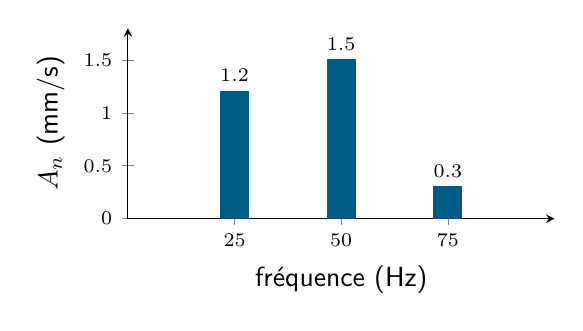
\begin{tikzpicture}
\begin{axis}[width=7cm, height=4cm, ybar, bar width=10pt, xlabel={fréquence (Hz)}, ylabel={$A_n$ (mm/s)},
  ymin=0, ymax=1.8, xmin=0, xmax=100, xtick={25,50,75}, axis lines=left, nodes near coords,
  every node near coord/.append style={font=\scriptsize}, tick label style={font=\scriptsize}]
  \addplot[fill=uimmblue, draw=uimmblue] coordinates {(25,1.2)(50,1.5)(75,0.3)};
\end{axis}
\end{tikzpicture}
\end{center}
\q{d)} La raie 2× ($50$\,Hz) domine, devant la raie 1× : on suspecte un \textbf{désalignement}.
\end{correction}

\begin{correction}[-- Exercice 7 : signal top-tour]
\source{exo:7}{\cours{meth:coefficients} (méthode et exemple du créneau)}
\q{a)} Le signal alterne $24$\,V et $0$\,V par demi-période. Valeur moyenne lue : $12$\,V.

\q{b)} $a_0 = \dfrac1T\displaystyle\int_0^{T/2}E\,\mathrm dt = \dfrac E2 = 12$\,V.
\[
a_n = \frac2T\int_0^{T/2}E\cos(n\omega t)\,\mathrm dt = \frac{2E}{Tn\omega}\big[\sin(n\omega t)\big]_0^{T/2} = \frac{E}{n\pi}\sin(n\pi) = 0.
\]
\[
b_n = \frac2T\int_0^{T/2}E\sin(n\omega t)\,\mathrm dt = \frac{2E}{Tn\omega}\big[-\cos(n\omega t)\big]_0^{T/2} = \frac{E}{n\pi}\big(1 - (-1)^n\big)
= \begin{cases} 0 & n \text{ pair}\\[2pt] \dfrac{2E}{n\pi} = \dfrac{48}{n\pi} & n \text{ impair}\end{cases}
\]
\q{c)} $f(t) \approx 12 + 15{,}28\sin(\omega t) + 5{,}09\sin(3\omega t) + 3{,}06\sin(5\omega t) + \cdots$

\q{d)} $f - \frac E2$ vaut $+\frac E2$ puis $-\frac E2$ : c'est le créneau impair du cours avec $\frac E2$ à la place de $E$. Sa série est $\frac{4}{\pi}\cdot\frac E2\sum\frac{\sin((2k+1)\omega t)}{2k+1} = \frac{2E}{\pi}\sum\dots$ : on retrouve les $b_n$ ci-dessus. Ajouter une constante ne modifie que $a_0$.
\end{correction}

\begin{correction}[-- Exercice 8 : le créneau décalé d'un quart de période]
\source{exo:8}{\cours{th:simplification}}
\q{a)} La courbe est symétrique par rapport à l'axe des ordonnées : $g$ est paire, donc $b_n = 0$. De plus $a_0 = 0$ (autant de temps à $+E$ qu'à $-E$).

\q{b)} $g$ est paire, donc $a_n = \frac4T\int_0^{T/2}g(t)\cos(n\omega t)\,\mathrm dt$, avec $g = E$ sur $\left[0\,;\,\frac T4\right[$ et $g = -E$ sur $\left]\frac T4\,;\,\frac T2\right]$ : c'est l'expression demandée. Comme $n\omega\frac T4 = \frac{n\pi}{2}$ et $n\omega\frac T2 = n\pi$ :
\[
\int_0^{T/4}\cos(n\omega t)\,\mathrm dt = \frac{\sin\left(\frac{n\pi}{2}\right)}{n\omega},
\qquad
\int_{T/4}^{T/2}\cos(n\omega t)\,\mathrm dt = \frac{\sin(n\pi) - \sin\left(\frac{n\pi}{2}\right)}{n\omega} = -\frac{\sin\left(\frac{n\pi}{2}\right)}{n\omega}.
\]
D'où $a_n = \dfrac{4E}{T}\times\dfrac{2\sin\left(\frac{n\pi}{2}\right)}{n\omega} = \dfrac{8E}{2n\pi}\sin\left(\dfrac{n\pi}{2}\right) = \dfrac{4E}{n\pi}\sin\left(\dfrac{n\pi}{2}\right)$.

\q{c)} $a_1 = \dfrac{4E}{\pi}$ ; $a_2 = 0$ ; $a_3 = -\dfrac{4E}{3\pi}$ ; $a_4 = 0$ ; $a_5 = \dfrac{4E}{5\pi}$.

\q{d)} $A_n = |a_n|$ : mêmes amplitudes que le créneau impair ($\frac{4E}{n\pi}$ pour $n$ impair). Décaler un signal dans le temps change les phases, pas le spectre d'amplitude. C'est pour cela que l'analyseur donne le même spectre quel que soit l'instant de déclenchement de la mesure.
\end{correction}

\begin{correction}[-- Exercice 9 : vidange d'une trémie]
\source{exo:9}{\cours{ex:rampe}}
\q{a)} Dent de scie descendante. $a_0 = \dfrac1T\displaystyle\int_0^T A\left(1 - \frac tT\right)\mathrm dt = \dfrac AT\left[t - \dfrac{t^2}{2T}\right]_0^T = \dfrac A2$.

\q{b)} $b_n = \dfrac{2A}{T}\left(\displaystyle\int_0^T\sin(n\omega t)\,\mathrm dt - \frac1T\int_0^T t\sin(n\omega t)\,\mathrm dt\right)$. La première intégrale est nulle (sinus sur un nombre entier de périodes). Par parties (calcul du cours), $\int_0^T t\sin(n\omega t)\,\mathrm dt = -\frac{T}{n\omega}$. Donc
\[
b_n = \frac{2A}{T}\times\left(-\frac1T\right)\times\left(-\frac{T}{n\omega}\right) = \frac{2A}{Tn\omega} = \frac{A}{n\pi}.
\]
\q{c)} $h(t) = \dfrac A2 + \dfrac A\pi\displaystyle\sum_{n\geq1}\frac{\sin(n\omega t)}{n}$. C'est la dent de scie du cours avec le signe des sinus inversé : $h = A - f$, donc $h$ a la même moyenne et des $b_n$ opposés.
\end{correction}

\begin{correction}[-- Exercice 10 : profil de came]
\source{exo:10}{\cours{ex:triangle} et \annexe{fiche:geogebra}}
\q{a)} $c$ est paire : $b_n = 0$. $a_0$ = moyenne = $2$\,mm (le triangle oscille entre $0$ et $4$, aire d'un triangle).

\q{b)} Ici $\omega = \frac{2\pi}{0{,}5} = 4\pi$. Le calcul formel de $8\int_0^{0{,}25}(4-16t)\cos(4n\pi t)\,\mathrm dt$ donne une expression en $\sin(n\pi)$ et $\cos(n\pi)$ qui se simplifie en
\[
a_n = \frac{8}{n^2\pi^2}\big(1 - (-1)^n\big) = \begin{cases} 0 & n \text{ pair}\\[2pt] \dfrac{16}{n^2\pi^2} & n \text{ impair.}\end{cases}
\]
\q{c)} La calculatrice donne $8\int_0^{0{,}25}(4-16x)\cos(4\pi x)\,\mathrm dx\approx 1{,}6211$ et $\frac{16}{\pi^2}\approx 1{,}6211$.

\q{d)} Oui : $c = 2 + (\text{triangle } \pm 2)$. Avec $E = 2$, le cours donne $a_n = \frac{8\times 2}{n^2\pi^2} = \frac{16}{n^2\pi^2}$ : même résultat, et la constante $2$ est $a_0$.
\end{correction}

% ============================================================
\needspace{8cm}
\section{Convergence et identification}

\begin{correction}[-- Exercice 11 : reconstituer le signal top-tour]
\source{exo:11}{\cours{th:dirichlet} et \annexe{fiche:geogebra}}
\q{a) b)} Plus $N$ augmente, plus la somme partielle épouse les paliers $0$ et $24$\,V ; il subsiste un petit dépassement près des sauts (phénomène de Gibbs).

\q{c)} $S(0) = 12 + \sum\frac{48}{\pi(2k-1)}\sin(0) = 12$ pour tout $N$. En $t = 0$, le signal saute de $0$ à $24$\,V : Dirichlet annonce la convergence vers $\frac{0 + 24}{2} = 12$.

\q{d)} $\sin\left((2k-1)\frac{\pi}{2}\right)$ vaut $1$, $-1$, $1$\dots\ \quad $N = 1$ : $S\left(\frac14\right) = 12 + \frac{48}{\pi}\approx 27{,}28$. \quad $N = 3$ : $S\left(\frac14\right) = 12 + \frac{48}{\pi}\left(1 - \frac13 + \frac15\right)\approx 25{,}24$.\\
$f$ est continue en $\frac14$ et vaut $24$ : $S\left(\frac14\right)$ doit tendre vers $24$.
\end{correction}

\begin{correction}[-- Exercice 12 : associer signaux et développements]
\source{exo:12}{\cours{meth:identifier}}
\begin{itemize}
  \item (1) créneau top-tour $0/E$ : moyenne $\frac E2$, sauts (termes en $\frac1n$), $f - \frac E2$ impaire (sinus seulement) : \textbf{(b)}.
  \item (2) dent de scie $0/A$ : moyenne $\frac A2$, sauts (en $\frac1n$), tous les harmoniques présents : \textbf{(c)}.
  \item (3) triangle pair $\pm E$ : pair (cosinus), moyenne nulle, continu (en $\frac1{n^2}$) : \textbf{(a)}.
\end{itemize}
Le développement (d) (cosinus en $\frac1n$, moyenne nulle) est celui du créneau pair de l'exercice 8 ; il ne correspond à aucun des trois signaux.
\end{correction}

% ============================================================
\needspace{8cm}
\section{Parseval et valeur efficace}

\begin{correction}[-- Exercice 13 : valeur efficace du triangle]
\source{exo:13}{\cours{th:parseval} et \cours{ex:parsevalcreneau}}
\q{a)} $f^2$ est paire : $\frac1T\int_0^T f^2 = \frac2T\int_0^{T/2}E^2\left(1-\frac{4t}T\right)^2\mathrm dt$. Avec $u = 1 - \frac{4t}{T}$, $\mathrm dt = -\frac T4\,\mathrm du$, et $u$ va de $1$ à $-1$ :
\[
\frac1T\int_0^T f^2(t)\,\mathrm dt = \frac2T\times E^2\times\frac T4\int_{-1}^{1}u^2\,\mathrm du = \frac{E^2}{2}\times\frac23 = \frac{E^2}{3},
\qquad
F_{\text{eff}} = \frac{E}{\sqrt3}\approx 0{,}577\,E.
\]
\q{b)} Fondamental seul : $\frac12a_1^2 = \frac12\left(\frac{8E}{\pi^2}\right)^2 = \frac{32E^2}{\pi^4}\approx 0{,}3285\,E^2$, soit $\frac{0{,}3285}{0{,}3333}\approx 98{,}6\,\%$ de la puissance. Le triangle est presque une sinusoïde (comparer aux $81\,\%$ du créneau).

\q{c)} Parseval : $\frac{E^2}{3} = \frac12\sum_{k\geq0}\frac{64E^2}{\pi^4(2k+1)^4}$, d'où $\displaystyle\sum_{k\geq0}\frac{1}{(2k+1)^4} = \frac{2\pi^4}{3\times 64} = \frac{\pi^4}{96}\approx 1{,}0147$.
\end{correction}

\begin{correction}[-- Exercice 14 : niveau global vibratoire]
\source{exo:14}{\cours{ex:niveauglobal}}
\q{a)} Valeurs efficaces des raies : $\frac{1{,}2}{\sqrt2}\approx 0{,}849$ ; $\frac{1{,}5}{\sqrt2}\approx 1{,}061$ ; $\frac{0{,}3}{\sqrt2}\approx 0{,}212$ (mm/s).
\[
V_{\text{eff}} = \sqrt{\frac{1{,}2^2 + 1{,}5^2 + 0{,}3^2}{2}} = \sqrt{1{,}89}\approx 1{,}37 \text{ mm/s.}
\]
\q{b)} $1{,}37 < 1{,}8$ : pas d'alerte. La raie 2× dominante justifie toutefois de planifier un contrôle d'alignement.

\q{c)} Nouvelle amplitude 2× : $0{,}375$\,mm/s. $V_{\text{eff}}' = \sqrt{\dfrac{1{,}44 + 0{,}140\,625 + 0{,}09}{2}}\approx 0{,}91$\,mm/s. Baisse : $\dfrac{1{,}37 - 0{,}91}{1{,}37}\approx 33\,\%$.
\begin{piege}
\textbf{Erreur fréquente :} diviser le niveau global par $4$. Seule une raie change : on recalcule la somme des carrés.
\end{piege}
\end{correction}

% ============================================================
\needspace{8cm}
\section{Problème de synthèse}

\begin{correction}[-- Problème : signature d'un défaut de roulement]
\source{exo:pb}{\cours{th:simplification}, \cours{def:spectre} et \cours{th:parseval}}
\q{1. a)} $T = \frac{1}{100} = 0{,}01$\,s $= 10$\,ms ; $\tau = 1$\,ms. Le signal est une suite d'impulsions de hauteur $E$ et de largeur $1$\,ms, centrées en $0$, $10$, $20$\dots\,ms.

\q{1. b)} Symétrique par rapport à l'axe des ordonnées : $s$ est paire, donc $b_n = 0$.

\q{2. a)} $a_0 = \frac1T\int_{-\tau/2}^{\tau/2}E\,\mathrm dt = \frac{E\tau}{T} = \frac{E}{10}$ : valeur moyenne du modèle. (Une accélération réelle est de moyenne nulle : c'est une limite de ce modèle simplifié.)

\q{2. b)} $a_n = \frac4T\int_0^{\tau/2}E\cos(n\omega t)\,\mathrm dt = \frac{4E}{Tn\omega}\sin\left(n\omega\frac\tau2\right)$. Or $Tn\omega = 2n\pi$ et $n\omega\frac\tau2 = \frac{n\pi\tau}{T} = \frac{n\pi}{10}$, d'où $a_n = \frac{2E}{n\pi}\sin\left(\frac{n\pi}{10}\right)$.

\q{2. c)} En multiples de $E$ (raies à $100$, $200$, \dots, $1\,000$\,Hz) :
\begin{center}
\renewcommand{\arraystretch}{1.3}
\begin{tabular}{|c|c|c|c|c|c|c|c|c|c|c|}
\hline
\rowcolor{uimmlightblue}
$n$ & $1$ & $2$ & $3$ & $4$ & $5$ & $6$ & $7$ & $8$ & $9$ & $10$ \\
\hline
$a_n$ & $0{,}197$ & $0{,}187$ & $0{,}172$ & $0{,}151$ & $0{,}127$ & $0{,}101$ & $0{,}074$ & $0{,}047$ & $0{,}022$ & $0$ \\
\hline
\end{tabular}
\end{center}
\begin{center}
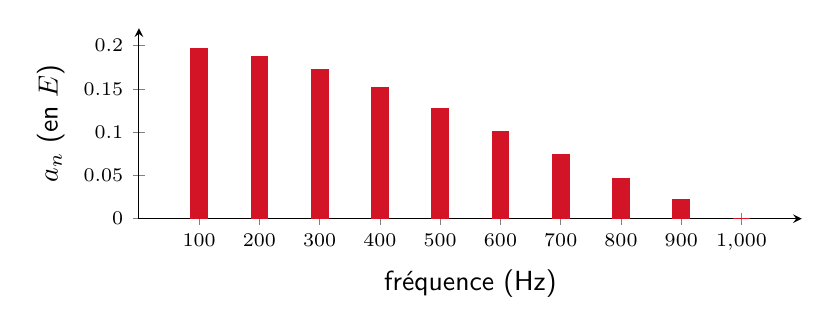
\begin{tikzpicture}
\begin{axis}[width=10cm, height=4cm, ybar, bar width=6pt, xlabel={fréquence (Hz)}, ylabel={$a_n$ (en $E$)},
  ymin=0, ymax=0.22, xmin=0, xmax=1100, xtick={100,200,300,400,500,600,700,800,900,1000}, axis lines=left,
  tick label style={font=\scriptsize}, scaled y ticks=false, yticklabel style={/pgf/number format/fixed}]
  \addplot[fill=uimmred, draw=uimmred] coordinates {(100,0.1967)(200,0.1871)(300,0.1717)(400,0.1514)(500,0.1273)(600,0.1009)(700,0.0736)(800,0.0468)(900,0.0219)(1000,0)};
\end{axis}
\end{tikzpicture}
\end{center}

\q{3. a)} Un balourd donne une seule raie (1×). Ici, les chocs produisent une série de raies régulièrement espacées de $f_c = 100$\,Hz, qui décroissent lentement : un « peigne ». Repérer l'espacement du peigne donne la fréquence des chocs, donc l'élément défectueux.

\q{3. b)} $\frac1T\int_0^T s^2 = \frac{E^2\tau}{T} = 0{,}1\,E^2$. Avec $a_0$ et les $9$ premiers harmoniques : $a_0^2 + \frac12\sum_{n=1}^{9}a_n^2\approx 0{,}0903\,E^2$, soit environ $90\,\%$ de la puissance. Il faut beaucoup d'harmoniques pour décrire un choc bref.

\q{3. c)} Avec $\tau = \frac{T}{20}$, $a_n = \frac{2E}{n\pi}\sin\left(\frac{n\pi}{20}\right)$ : le premier zéro passe au rang $20$ ($2\,000$\,Hz). Plus le choc est bref, plus son énergie s'étale vers les hautes fréquences. Un défaut de roulement naissant produit des chocs brefs et faibles, noyés à basse fréquence dans les raies de rotation : on le cherche plutôt dans le domaine des hautes fréquences.
\end{correction}

\end{document}
